\chapter{Moteur d'Extraction des Descripteurs Visuels}
\label{chap:descripteurs}

\section{Architecture du Moteur d'Extraction : \texttt{DescriptorEngine}}

L'efficacité et la reproductibilité d'un système CBIR reposent sur la rigueur de son moteur de caractérisation visuelle. Dans Perceptra, cette responsabilité est dévolue à la classe sans état \texttt{DescriptorEngine} (\texttt{src/services/descriptor\_engine.py}).

Conçu pour fonctionner de manière strictement déterministe, le moteur reçoit en entrée le flux brut d'octets (\textit{raw bytes}) d'une image matricielle et produit en sortie un dictionnaire structuré contenant les hyperparamètres d'extraction, les données statistiques détaillées et le vecteur numérique normalisé prêt pour l'indexation.

\begin{figure}[H]
\centering
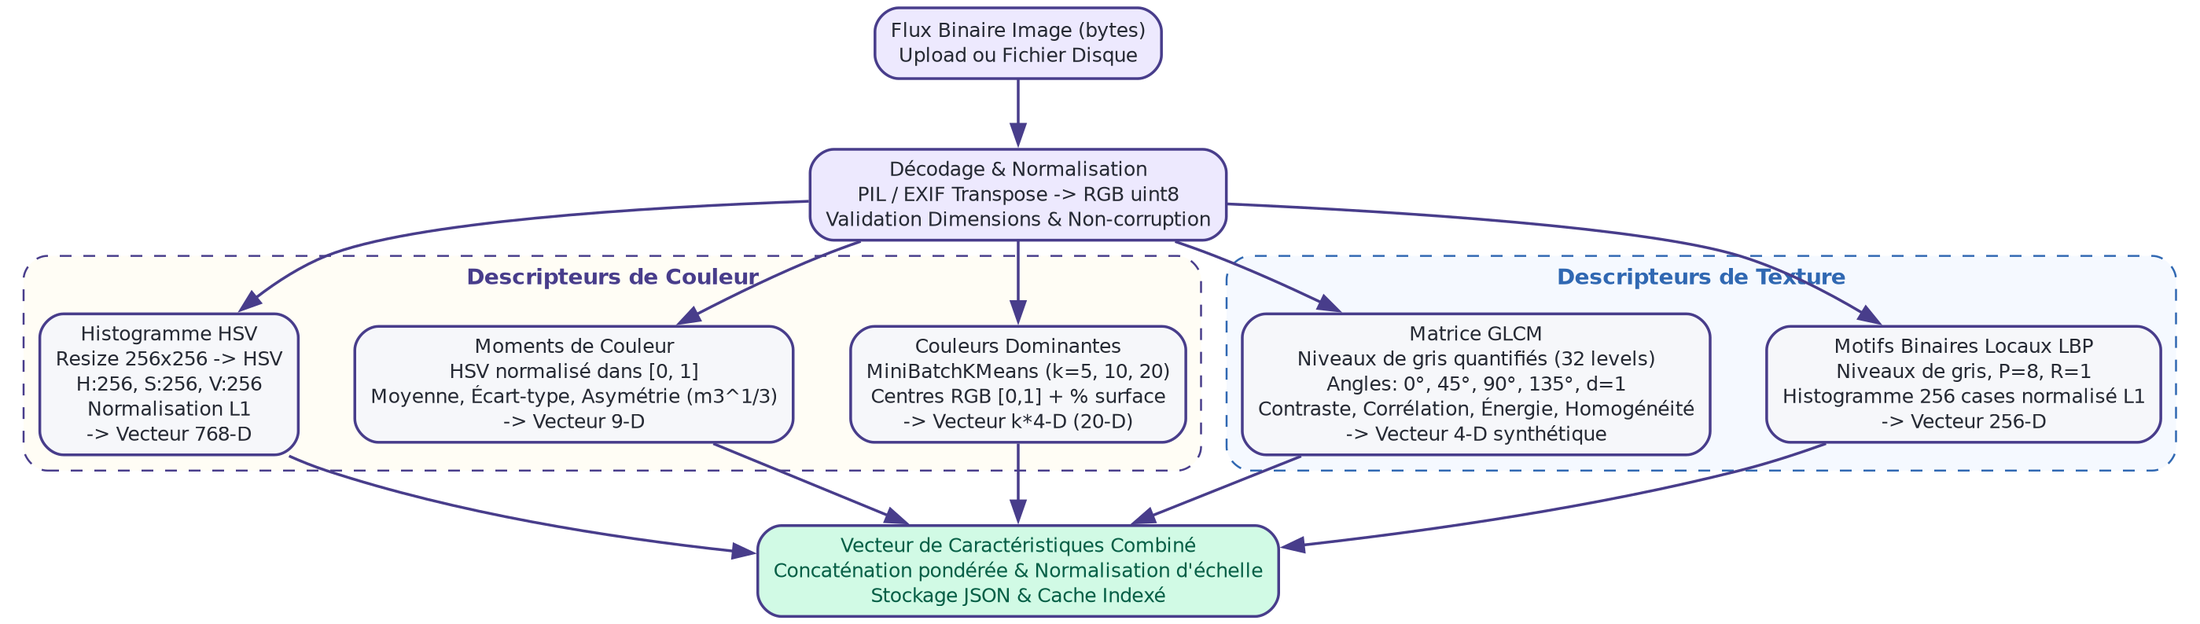
\includegraphics[width=0.78\textwidth]{images/05-pipeline-extraction-descripteurs.png}
\caption{Pipeline d'extraction multi-facettes et construction de la signature visuelle}
\label{fig:pipeline_descripteurs}
\end{figure}

Avant toute opération de filtrage, la méthode statique \texttt{decode\_image\_rgb} procède à un prétraitement unifié~:
\begin{enumerate}
    \item \textbf{Correction d'orientation EXIF~:} Application de \texttt{ImageOps.exif\_transpose} afin que les images issues d'appareils mobiles ou reflex soient redressées dans leur orientation physique réelle sans biais angulaire.
    \item \textbf{Normalisation d'espace colorimétrique~:} Conversion systématique en format RGB non compressé sous forme de tableau NumPy de type \texttt{uint8} à trois canaux de forme $(H, W, 3)$.
    \item \textbf{Contrôle de conformité~:} Rejet immédiat de tout flux vide ou corrompu par la levée de l'exception typée \texttt{InvalidImageStreamError}.
\end{enumerate}

\section{Descripteurs de Couleur}

La couleur traduit la composition spectrale d'une scène. Perceptra combine trois descripteurs complémentaires offrant des niveaux d'abstraction variés.

\subsection{1. Histogramme de Couleur HSV 768-D Normalisé L1}
Bien que le format d'acquisition soit usuellement le RGB, les trois composantes sont hautement corrélées entre elles et sensibles aux variations d'éclairement. Nous procédons donc à une conversion dans l'espace \textbf{HSV} (\textit{Teinte, Saturation, Valeur}).

L'image est d'abord rééchantillonnée en dimensions normalisées $256 \times 256$ pixels par interpolation \texttt{cv2.INTER\_AREA} afin d'uniformiser la complexité algorithmique. Ensuite, les histogrammes individuels pour chaque canal sont calculés via \texttt{cv2.calcHist}~:
\begin{itemize}
    \item Canal $H$ (Teinte) : quantifié sur 256 intervalles dans la plage $[0, 180[$~;
    \item Canal $S$ (Saturation) : quantifié sur 256 intervalles dans la plage $[0, 256[$~;
    \item Canal $V$ (Valeur) : quantifié sur 256 intervalles dans la plage $[0, 256[$.
\end{itemize}

Afin de conférer au descripteur une invariance stricte à l'échelle de l'image, chaque canal subit une \textbf{normalisation $L_1$} indépendante~:
\begin{equation}
\tilde{h}_c(k) = \frac{h_c(k)}{\sum_{i=0}^{255} h_c(i)}, \quad \forall c \in \{H, S, V\}, \quad k \in [0, 255]
\end{equation}

Les trois vecteurs normalisés de 256 dimensions sont concaténés pour former une signature chromatique globale de \textbf{768 dimensions}~:
\begin{equation}
\mathbf{v}_{\text{hist}} = \big[ \tilde{h}_H(0), \dots, \tilde{h}_H(255), \; \tilde{h}_S(0), \dots, \tilde{h}_S(255), \; \tilde{h}_V(0), \dots, \tilde{h}_V(255) \big] \in \mathbb{R}^{768}
\end{equation}

\subsection{2. Moments Statistiques de Couleur 9-D (Stricker \& Orengo)}
Pour obtenir une représentation extrêmement compacte et robuste au bruit haute fréquence, nous calculons les trois premiers moments statistiques de distribution selon le formalisme de Stricker et Orengo~\cite{stricker1995similarity}.

Les canaux HSV sont au préalable normalisés dans l'intervalle continu $[0, 1]$ ($H$ divisé par 179, $S$ et $V$ divisés par 255). Pour chaque canal $c \in \{H, S, V\}$ de $N$ pixels, les moments sont définis par~:
\begin{enumerate}
    \item \textbf{Moyenne $\mu_c$~:} $\mu_c = \frac{1}{N} \sum_{i=1}^{N} p_{c, i}$
    \item \textbf{Écart-type $\sigma_c$~:} $\sigma_c = \sqrt{\frac{1}{N} \sum_{i=1}^{N} (p_{c, i} - \mu_c)^2}$
    \item \textbf{Asymétrie signée $s_c$~:} Pour préserver le signe lors de l'extraction de la racine cubique~:
    \begin{equation}
    m_{3, c} = \frac{1}{N} \sum_{i=1}^{N} (p_{c, i} - \mu_c)^3, \quad s_c = \operatorname{sign}(m_{3, c}) \cdot \sqrt[3]{|m_{3, c}|}
    \end{equation}
\end{enumerate}

Le vecteur résultant compile ces 9 valeurs réelles~:
\begin{equation}
\mathbf{v}_{\text{moments}} = [\mu_H, \sigma_H, s_H, \; \mu_S, \sigma_S, s_S, \; \mu_V, \sigma_V, s_V] \in \mathbb{R}^9
\end{equation}

\subsection{3. Couleurs Dominantes par Partitionnement MiniBatchKMeans}
L'algorithme \texttt{MiniBatchKMeans} est appliqué sur l'image sous-échantillonnée ($128 \times 128$) avec $k=5$ centroïdes RGB et une graine aléatoire fixe (\texttt{random\_state=42}). Pour chaque centroïde $j \in [1, 5]$ ordonné par poids volumique $w_j \in [0, 1]$, la composante vectorielle compile les couleurs normalisées et la surface~:
\begin{equation}
\mathbf{c}_j = \left[ \frac{\bar{R}_j}{255}, \; \frac{\bar{G}_j}{255}, \; \frac{\bar{B}_j}{255}, \; w_j \right] \implies \mathbf{v}_{\text{dom}} \in \mathbb{R}^{20}
\end{equation}

\section{Descripteurs de Texture}

\subsection{1. Matrice de Co-occurrence de Niveaux de Gris (GLCM)}
L'image en niveaux de gris est quantifiée linéairement sur $L=32$ niveaux d'intensité. Pour une distance $d=1$ selon les quatre angles $\theta \in \{0^\circ, 45^\circ, 90^\circ, 135^\circ\}$, les quatre métriques de Haralick et al.~\cite{haralick1973textural} sont évaluées~:
\begin{align}
\text{Contraste~:} \quad & f_{\text{con}}(\theta) = \sum_{i=0}^{L-1}\sum_{j=0}^{L-1} (i - j)^2 P_{\theta}(i, j) \\
\text{Corrélation~:} \quad & f_{\text{corr}}(\theta) = \sum_{i=0}^{L-1}\sum_{j=0}^{L-1} \frac{(i - \mu_i)(j - \mu_j) P_{\theta}(i, j)}{\sigma_i \sigma_j} \\
\text{Énergie (ASM)~:} \quad & f_{\text{ene}}(\theta) = \sum_{i=0}^{L-1}\sum_{j=0}^{L-1} P_{\theta}(i, j)^2 \\
\text{Homogénéité~:} \quad & f_{\text{hom}}(\theta) = \sum_{i=0}^{L-1}\sum_{j=0}^{L-1} \frac{P_{\theta}(i, j)}{1 + (i - j)^2}
\end{align}

Le vecteur synthétique $\mathbf{v}_{\text{glcm}} \in \mathbb{R}^4$ compile ces quatre grandeurs moyennées sur les 4 orientations, conférant une invariance stricte aux rotations planes.

\subsection{2. Motifs Binaires Locaux (LBP -- Local Binary Patterns)}
Pour chaque pixel central $g_c$, nous considérons ses $P=8$ voisins équidistants à rayon $R=1$~:
\begin{equation}
LBP_{P, R}(x_c, y_c) = \sum_{p=0}^{P-1} s(g_p - g_c) \cdot 2^p, \quad \text{où } s(z) = \begin{cases} 1 & \text{si } z \ge 0 \\ 0 & \text{si } z < 0 \end{cases}
\end{equation}
L'histogramme des 256 occurrences est normalisé par la somme totale ($L_1$), produisant $\mathbf{v}_{\text{lbp}} \in \mathbb{R}^{256}$.

\begin{table}[H]
\centering
\rowcolors{2}{LightGray}{white}
\begin{tabularx}{\textwidth}{>{\bfseries}p{3.5cm}p{1.8cm}p{2.5cm}X}
\toprule
\rowcolor{TableHeader}
\color{white}Nom du Descripteur & \color{white}Dim. & \color{white}Espace / Entrée & \color{white}Propriétés Clés \\
\midrule
\texttt{color\_histogram} & 768 & HSV ($256 \times 3$) & Normalisation L1 par canal, robuste aux variations lumineuses. \\
\texttt{color\_moments} & 9 & HSV norm. $[0, 1]$ & Moyenne, écart-type et asymétrie signée $\sqrt[3]{m_3}$ ; très compact. \\
\texttt{dominant\_colors} & 20 & RGB ($k=5$) & 5 centroïdes RGB ordonnés par importance avec pourcentages surfaciques. \\
\texttt{glcm} & 4 & Niveaux de gris (32) & Contraste, corrélation, énergie et homogénéité moyennés sur 4 angles. \\
\texttt{lbp\_histogram} & 256 & Niveaux de gris & Voisinage $P=8, R=1$, histogramme L1 décrivant la micro-texture locale. \\
\bottomrule
\end{tabularx}
\caption{Synthèse dimensionnelle et caractéristiques des descripteurs de Perceptra}
\label{tab:descripteurs_synthese}
\end{table}
